\chapter{Partition Forests}
\label{chap:ipfs}

%---
\section{Chapter Overview}

In Chapter~\ref{chap:methodology}, I discussed the goals of my doctorate and the methods I chose to try to achieve them. This chapter introduces partition forests as a hierarchical representation for aggregate objects in general, and images in particular. I present a hierarchy of novel editing algorithms for partition forests, and propose partition forest selection and partition forest multi-feature selection data structures to support subtree-based selection and identification of nodes within forests. I further show how these features can be integrated into a graphical user interface for working with image partition forests (that is, partition forests in an imaging context). This lays the foundation for the following two chapters, which describe how partition forests can be constructed from images (Chapter~\ref{chap:segmentation}) and then used to identify features therein (Chapter~\ref{chap:featureid}).

%---
\section{What is a Partition Forest?}

\subsection{Concept}

A partition forest is in essence a hierarchy of adjacency graphs that all partition the same object (the sense in which a graph can partition an object will be formalised in \S\ref{sec:ipfs-definition}). The object itself can be anything that can be divided into pieces, whether that be an image, a road network or an organisation. As was seen in \S\ref{sec:background-partitionhierarchies}, partition forests (whether called by that name or otherwise) have been widely used as a hierarchical representation for images. However, surprisingly little attention has been devoted to how to edit them post-construction (with perhaps the notable exception being Nacken's work in \cite{nacken95}).

\newpage

The key components that make up a partition forest are illustrated in Figure~\ref{fig:ipfs-concept}, which shows a partition forest that might be constructed for a simple $4 \times 4$ image. A forest is made up of a number of layers, each of which is an adjacency graph representing a partition of an object (in this case, the image). Each partition is refined by the next highest partition, in the sense that each node in partition $i+1$ is the union of some of the nodes in partition $i$.

The nodes in each layer represent groups of the smallest sub-objects into which the represented object can be divided (in this case, each node represents an image region, consisting of a group of pixels), and can have layer-dependent properties associated with them (shown as blue text in the figure). Properties of nodes in the leaf layer can be assigned arbitrarily, but properties of nodes in branch layers must be functions of the properties of their children in the layer below (this will be defined formally in \S\ref{sec:ipfs-definition}). In this example, a single, arbitrary value has been associated with each node in the leaf layer of the forest. Nodes in higher layers have been given a `mean value' property that is calculated from the values of the subsumed leaf nodes.

Each layer also contains edges between nodes that are in some sense adjacent (in the case of images, this is defined in such a way that the nodes are considered adjacent if their corresponding regions are adjacent in the image). Each edge has an associated value (shown as underlined text in the figure). The values on the edges in the leaf layer can be assigned according to any scheme desired -- in this example, they represent the height of the `lowest pass point' between adjacent nodes, based on the values associated with the pixels. The value on an edge between a pair of nodes in a branch layer must be a function of the values on any edges between their respective children in the layer below (again, this will be defined formally in \S\ref{sec:ipfs-definition}). In this example, the value on an edge between two nodes, $u$ and $v$, in a branch layer is calculated to be the smallest value on any edge between a child of $u$ and a child of $v$, in keeping with the lowest pass idea above.

In addition to the forest layers themselves, a partition forest also contains forest links that join the nodes in adjacent layers together (the coloured, dashed lines in the figure). In particular, there is a link between each node and the node that contains it in the layer above. These links naturally define parent/child relationships between forest nodes.

%---
\stufigex{height=24cm}{ipfs/ipfs-concept.png}{The concept of a partition forest (see main text for discussion)}{fig:ipfs-concept}{p}
%---

\subsection{Definition}
\label{sec:ipfs-definition}

It is possible to define partition forests more formally as follows:

\begin{definition}
An \textbf{object} is a non-empty set of basic components which together form a contiguous whole. (For example, a contiguous image region would be a non-empty set of pixels.)
\end{definition}

\begin{definition}
A set of k objects $\{o'_1,\ldots,o'_k\}$ \textbf{partitions} an object $o$ iff $\bigcup_i o'_i = o$ and $\forall i,j \cdot o'_i \cap o'_j = \emptyset$. We write the relation as $\mathcal{P}(\{o'_1,\ldots,o'_k\}, o)$.
\end{definition}

\begin{definition}
Given an object $o$, and two objects sets $O'_f = \{o'_{f1},\ldots,o'_{fk_f}\}$ and $O'_c = \{o'_{c1},\ldots,o'_{ck_c}\}$, satisfying $\mathcal{P}(O'_f,o)$ and $\mathcal{P}(O'_c,o)$, we say that $O'_c$ is a \textbf{coarser partition} of $o$ than $O'_f$ (written $O'_f \sqsubseteq O'_c$) iff for every object $o'_{ci} \in O'_c$ there exists a subset $S_i \subseteq O'_f$ such that $\mathcal{P}(S_i,o'_{ci})$. (In other words, $O'_f$ is a partition of $o$ in which each individual object in $O'_c$ has itself been partitioned.)
\end{definition}

\begin{definition}
Letting $\mbox{adj}_o(o'_i, o'_j)$ denote that sub-objects $o'_i$ and $o'_j$ are (in some sense) adjacent in an object $o$, we define a \textbf{weight function} $w_o$ for $o$ to be a function of type $\mathbb{P}(o) \times \mathbb{P}(o) \to \mathbb{R}^+$ that satisfies the following two requirements:
%
\begin{enumerate}

\item $w_o(o'_i, o'_j) \ne \infty$ when, and only when, $adj_o(o'_i, o'_j)$ is true

\item Given any sets $S_i$ and $S_j$ satisfying $\mathcal{P}(S_i,o'_i)$ and $\mathcal{P}(S_j,o'_j)$, the value $w_o(o'_i, o'_j)$ is a function of only the values in the set $\{w_o(s_i, s_j) \; | \; s_i \in S_i, \; s_j \in S_j\}$.

\end{enumerate}

\end{definition}

\begin{definition}
A \textbf{property set} is an ordered set (a tuple) of properties, each of which is a function that maps an object to a value (the types of the values may differ). For example, in the context of imaging it would be possible to have an area property that calculates the area of a given image region in pixels.
\end{definition}

\begin{definition}
Given a property set $P = (p_1,\ldots,p_k)$ and an object $o$, the \textbf{property value set} $V_P(o)$ is the ordered set that results from applying each property in $P$ to the object $o$, namely $(p_1(o),\ldots,p_k(o))$.
\end{definition}

\begin{definition}
We call a property set $P$ \textbf{directly calculable} from a property set $P'$ iff, for any given set of sub-objects $O'$ and object $o$ satisfying $\mathcal{P}(O',o)$, the property value set $V_P(o)$ is a function of only the property value sets in $\{V_{P'}(o') \; | \; o' \in O'\}$. We write this relation as $P' \hookrightarrow P$.
\end{definition}

\begin{definition}
A \textbf{partition node} is a node in a partition forest. Each node $n$ represents a given object, denoted as $\mbox{obj}(n)$. The set of objects represented by a node set $N$ can be denoted as $\mbox{Objs}(N)$.
\end{definition}

\begin{definition}
A \textbf{partitioning graph} $G(N,w_o,P)$ of an object $o$ is an undirected graph with weighted edges and property values on each node. It has ordered node set $N$, satisfying $\mathcal{P}(\mbox{Objs}(N),o)$, edge set $E = \{(\{n_i,n_j\},w(\mbox{obj}(n_i),\mbox{obj}(n_j))) \; | \; n_i, n_j \in N \mbox{ and } n_i \ne n_j\}$, and property value set tuple $\textit{VS} = (V_P(\mbox{obj}(n)) \; | \; n \in N)$.
\end{definition}

\begin{definition}
Given:

%-
\begin{enumerate}

\item An object $o$
\item A non-empty tuple $\textit{NS} = (N_1,\ldots,N_k)$, where:

%--
\begin{enumerate}

\item $\forall N_i \in \textit{NS} \cdot \mathcal{P}(\mbox{Objs}(N_i),o)$
\item $\mbox{Objs}(N_1) \sqsubseteq \ldots \sqsubseteq \mbox{Objs}(N_k)$ 
\item $\forall n \in N_1 \cdot |\mbox{obj}(n)| = 1$

\end{enumerate}
%--

\item A weight function $w_o$ for $o$
\item A non-empty tuple $\textit{PS} = (P_1,\ldots,P_k)$ satisfying $P_1 \hookrightarrow \ldots \hookrightarrow P_k$

\end{enumerate}
%-

\noindent We define the \textbf{partition forest} $PF_{\textit{NS},w_o,\textit{PS}}(o)$ to be the pair $(\textit{FL},\textit{PG})$, in which:

\begin{itemize}

\item $\textit{FL}$ is a set of forest links, defined as:
%
\[
\{(n_c,n_p) \; | \; \exists i \in [1,k-1] \cdot n_c \in N_i \mbox { and } n_p \in N_{i+1} \mbox{ and } \mbox{obj}(n_c) \subseteq \mbox{obj}(n_p)\}
\]

\item $\textit{PG}$ is an ordered set of partitioning graphs of $o$, defined as:
%
\[
(G(N_1,w_o,P_1),\ldots,G(N_k,w_o,P_k))
\]

\end{itemize}

\end{definition}

\noindent We can also define a parent/child relation between nodes, namely that $p = \mbox{parent}(c)$ iff $(c,p) \in \textit{FL}$. (This is equivalent to saying $c \in \mbox{children}(p)$.)

%---
\section{Mutating Algorithms for Partition Forests}
\label{sec:ipfs-mutatingalgorithms}

Partition forests, as presented thus far, are a useful hierarchical representation for aggregate objects, but they are \emph{static}: that is, once a partition forest has been constructed for a given object, it does not change. This can be problematic, because constructing a perfect forest is potentially hard, and the number of possible forests for a given object is (at least theoretically) infinite. Even being more practical, and imposing the reasonable condition that every edge in the adjacency graph for the forest's leaf layer should have been elided (merging the two nodes it joins) by branch layer $E$, where $E$ is the total number of edges in the leaf adjacency graph, we can observe that there are still $E^2$ possible forests for an object (the $E^2$ comes from choosing a layer between $1$ and $E$ inclusive at which each leaf layer edge is removed by merging the nodes it joins). Putting this into context, that means that for a $4$-connected image of size $w \times h$, there are $(4wh - 2(w+h))^2$ possible partition forests (over a million possibilities for a $512 \times 512$ image). There is therefore a pressing need for mutating algorithms that allow us to transform one partition forest into another, in order to allow a user to work around potential issues with the initial partition forest construction. In this section, I present a hierarchy of novel algorithms (see Figure~\ref{?}) that allow users to edit partition forests, thereby changing them from being merely a static data structure into being a dynamic one.

\subsection{Core Algorithms}

In order to be able to transform a partition forest for an object $o$ into any other partition forest for $o$, a certain minimal set of forest operations must be possible. Specifically, it must be possible to clone and delete forest layers, and merge sibling forest nodes (nodes that share the same parent). To show that these are both necessary and sufficient, we first prove the following theorem:

\begin{theorem}
\label{thrm:ipfs-construction}
It is possible to construct any partition forest for a particular object by starting from the leaf layer and using only clone layer and merge sibling nodes operations. They are also the absolute minimum necessary.
\end{theorem}

\begin{proof}
(Sufficiency) Every branch node in the forest is the union of some of the nodes in the layer below (its children). To form each new layer of the forest, it therefore suffices to clone the current topmost layer (using clone layer) and merge the nodes which comprise each branch node (using merge sibling nodes). This can be repeated as many times as necessary to form the desired forest.
\end{proof}

\begin{proof}
(Necessity) Without the clone layer operation (or an equivalent way of creating new layers), it is impossible to create partition forests with more than one layer. Without the merge sibling nodes operation (or an equivalent way of merging nodes in a given layer), it is impossible to create non-trivial branch nodes. $\Box$
\end{proof}

\noindent Given this, it is simple to extend it to transformations between arbitrary partition forests over the same object:

\begin{theorem}
\label{thrm:ipfs-transformation}
It is possible to transform any partition forest $F$ for a particular object into any other partition forest $F'$ for the same object using only clone layer, delete layer and merge sibling nodes operations. They are also the absolute minimum necessary.
\end{theorem}

\begin{proof}
(Sufficiency) Trivial: it suffices to delete all the branch layers in $F$ and apply Theorem~\ref{thrm:ipfs-construction} to construct $F'$.
\end{proof}

\begin{proof}
(Necessity) Without the clone layer operation, it is impossible to transform to a forest with more layers than currently present. Without the delete layer operation, it is impossible to transform to a forest with fewer layers than currently present. Without the merge sibling nodes operation, it is impossible to alter any of the layers. All three operations are thus individually necessary. $\Box$
\end{proof}

\noindent Theorem~\ref{thrm:ipfs-transformation} proves that only three core operations are strictly necessary to allow partition forests to be edited arbitrarily. However, in practice it is vitally important to also directly support node splitting as a core operation if efficient editing is desired (it is technically possible to split a node by reconstructing its entire layer, but this is clearly impractical). For this reason, the core partition forest algorithms are defined as (1) layer cloning, (2) layer deletion, (3) sibling node merging and (4) node splitting. Each of these operations is now examined in detail. Since they were ultimately designed for use as part of an interactive system for image analysis, a sample user interface for each operation is presented in that context (where relevant). The descriptions also focus not only on how each operation can be executed, but also on how it can be undone, and on what preconditions need checking before it is executed. When analysing the complexity of the algorithms, I make the following assumptions about the data structures used:

\begin{itemize}
\item The forest layers are stored in some sort of resizeable array (for example, a std::vector in C++).
\item The nodes in the forest's leaf layer are also stored in some sort of array (not necessarily resizeable). This makes particular sense for image partition forests, where the leaf layer contains the regular grid of pixels in the image.
\item The nodes in the forest's branch layers are stored in some sort of tree-based map (for example, a std::map in C++).
\item Edges in the leaf layer are created on-the-fly -- it would be unnecessarily costly to store all the edges between adjacent image pixels, for example.
\item Edges in other layers are stored using some sort of tree-based data structure (such as the multi-index container provided in C++'s Boost libraries).
\end{itemize}

\noindent All of these data structures are assumed to provide their usual complexity guarantees (e.g.~logarithmic lookup for tree-based maps, etc.)

\subsubsection{Layer Cloning}

\paragraph{Description}

New layers can be inserted anywhere in the forest by cloning the layer below the insertion point (for example, see Figure~\ref{fig:ipfs-algorithms-layercloning}). A partition forest is guaranteed to have at least one layer at all times, so there will always be an existing layer to clone. In terms of the earlier partition forest definition, this has the effect of inserting a copy of the partitioning graph into the set $\textit{PG}$, and adding to $\textit{FL}$ the appropriate forest links between nodes in the inserted layer and those in the layer(s) adjacent to it.

\paragraph{C++ Method Interface}

\begin{lstlisting}[style=Prototype]
void clone_layer(int indexB);
\end{lstlisting}

\paragraph{User Interface for Image Analysis}

The simplest user interface just allows the user to clone the current layer by (for example) clicking on a menu item (see Figure~\ref{fig:ipfs-algorithms-layercloning-gui}). After cloning the layer, the interface can display the clone so that the user can begin working with it immediately. An alternative would be to allow the user to clone any layer in the forest by displaying a dialog box allowing them to choose the layer to be cloned, but in my view the former approach is more intuitive.

%---
\stufigex{height=5cm}{ipfs/ipfs-algorithms-layercloning-gui.png}{The user interface for layer cloning: a simple menu item allowing the current layer to be cloned.}{fig:ipfs-algorithms-layercloning-gui}{p}
%---

\paragraph{Precondition Checking}

The only precondition that needs checking for layer cloning is that the clonee (the layer being cloned) exists. This can be trivially checked in $O(1)$ time. Note that if the clone layer command is invoked from the user interface, the layer will inevitably exist (and we can skip the check), since the layer currently being viewed exists by definition.

\paragraph{Executing the Command}

Pseudo-code to execute a clone layer command is shown in Listing~\ref{code:ipfs-forest-clonelayerimpl}. The essence of the approach taken is simple: clone the graph of the layer below, then update the forest links between the clone layer and the layers below and above it. In order to implement the algorithm efficiently, however, it is important to employ a sensible iterator-based interface to the nodes in each forest layer: this allows us to iterate over the nodes in a layer in linear time and avoid the costly node lookups that might otherwise be necessary. Thus, in the pseudo-code, we iterate simultaneously over the nodes in the clonee layer and the clone, first propagating each parent link from the clonee node up to the clone node, then linking the corresponding nodes in the clonee and the clone together.

TODO

%To analyse the complexity of the algorithm, we proceed as follows. Firstly, let $n_\ell$ be the number of nodes and $e_\ell$ be the number of adjacency graph edges in layer $\ell$. Suppose layer $c$ is to be inserted above layer $b$ and below layer $a$ (if it exists). Then evidently $n_c = n_b$ and $e_c = e_b$. The complexity of cloning $b$'s partitioning graph is $\Theta(e_b)$. (We observe in passing that $n_b \in O(e_b)$, since the adjacency graph is connected, so there is no need to include $n_b$ when analysing the complexity of the cloning process.) Forest links must then be added between layers $b$ and $c$, and $c$ and $a$, if $a$ exists. In either case, there is a constant amount of work to do for each of the $n_b$ nodes in layer $c$ (see pseudo-code), so the amount of work done updating the forest links is $\Theta(n_b)$. The overall complexity of the algorithm is thus $\Theta(e_b + n_b) = \Theta(e_b)$.

\begin{stulisting}[p]
\caption{Forest : Clone Layer Implementation}
\label{code:ipfs-forest-clonelayerimpl}
\begin{lstlisting}[style=Default]
function clone_layer_impl
: (indexB : int) $\to \emptyset$

	// Note: We denote the layer being cloned as B and insert the clone layer C
	// above it.

	// Clone the graph of the layer below to make a new layer and insert it.
	var layerB : ForestLayer := forest_layer(indexB);
	var layerC : BranchLayer := clone_graph(layerB);
	insert_branch_layer(indexB + 1, layerC);

	// Copy the parent links from layer B to layer C, then update the links between
	// B and C to make corresponding nodes in each link to each other.
	var bt : NodeIterator := layerB.nodes_begin();
	var bend : NodeIterator := layerB.nodes_end();
	var ct : BranchNodeIterator := layerC.branch_nodes_begin();
	var cend : BranchNodeIterator := layerC.branch_nodes_end();

	while ct $\ne$ cend
		ct.set_parent(bt.parent());
		bt.set_parent(bt.index());
		ct.set_children({bt.index()});
		bt := next(bt), ct := next(ct);

	listeners.layer_was_cloned(indexB);
\end{lstlisting}
\end{stulisting}

\paragraph{Undoing the Command}

A clone layer command can be undone by simply deleting the clone (see Listing~\ref{code:ipfs-forest-deletelayerimpl} for pseudo-code). The complexity of this is analysed in the next section.

\subsubsection{Layer Deletion}

\paragraph{Description}

Any layer except the lowest can be deleted from the hierarchy (for example, see Figure~\ref{fig:ipfs-algorithms-layerdeletion}). In terms of the partition forest definition, this has the effect of removing both the specified partitioning graph from $\textit{PG}$ and the forest links referencing the deleted layer from $\textit{FL}$, and adding new forest links where necessary between any layers on either side of the one being removed.

\paragraph{C++ Method Interface}

\begin{lstlisting}[style=Prototype]
void delete_layer(int indexD);
\end{lstlisting}

\paragraph{User Interface for Image Analysis}

As with layer cloning, the simplest user interface just allows the user to delete the current layer by clicking on a menu item (see Figure~\ref{fig:ipfs-algorithms-layerdeletion-gui}).

%---
\stufigex{height=5cm}{ipfs/ipfs-algorithms-layerdeletion-gui.png}{The user interface for layer deletion: a simple menu item allowing the current layer to be deleted.}{fig:ipfs-algorithms-layerdeletion-gui}{p}
%---

\paragraph{Precondition Checking}

The only precondition that needs checking for layer deletion is that the layer being deleted is a branch layer. This is trivial to check in $O(1)$ time. (Depending on the design of the overall application, it may be necessary to make layer deletion slightly more constrained. For instance, an application that shows only branch layers may want to prevent the user from deleting the last branch layer, even though it's perfectly fine when viewed strictly from a partition forest perspective. Regardless, though, the required checks remain trivial.)

\paragraph{Executing the Command}

Pseudo-code to execute a delete layer command is shown in Listing~\ref{code:ipfs-forest-deletelayerimpl}. The idea is to update the forest links between the layers on either side of the layer to be deleted and then remove the layer itself from the forest. Specifically, if $D$ is the layer being deleted, $B$ is the layer below it and $A$ is the layer above (if it exists), then each node in $B$ should have its parent link updated to point to its grandparent in layer $A$. The grandparent nodes in $A$ should similarly have their child links updated to point to their grandchildren in layer $B$. To implement this efficiently, it is important to avoid calculating the grandchildren of nodes in $A$ explicitly. This is most easily arranged by iterating over the grandchildren and updating the grandparents during the course of the iteration (see pseudo-code). It is important to return the deleted layer (unchanged) at the end of the process, because it must be cached if we are to support undo.

We use the same notation to analyse the complexity as in the layer cloning analysis. The first loop in the pseudo-code (which clears the child sets in layer $A$) does a constant amount of work for each node in layer $A$ and is thus $O(n_a)$. Each iteration of the second loop (which updates the forest links) does an $O(\log n_d)$ lookup in layer $D$ to find the grandparent of $n$, sets $n$'s parent in constant time and then potentially does an $O(\log n_a)$ lookup on layer $A$, followed by an insertion into the set of child nodes of the grandparent node. The overall work done by the loop excluding the final insertions is $O(n_b (\log n_d + \log n_a)) = O(n_b \log n_d)$, since $n_a \le n_d$. The cost of the insertions depends on the distribution of the child nodes and how they are stored. If child nodes are stored as resizeable arrays, then each insertion is amortized constant time and the total cost of all the insertions is amortized $O(n_b)$. (If, however, tree-based sets are used, and all the child nodes have the same grandparent, the total cost ends up being $O(\log n_b!)$, i.e.~the cost of inserting $n_b$ elements one by one into a tree-based set.) Assuming the former, the total amortized complexity of the second loop is $O(n_b \log n_d) + O(n_b) = O(n_b \log n_d)$. Finally, the complexity of actually erasing the layer from the forest is amortized constant time. The total amortized complexity of the algorithm as a whole is therefore $O(n_a) + O(n_b \log n_d) + O(1) = O(n_b \log n_d)$, since $n_a \le n_b$.

\begin{stulisting}[p]
\caption{Forest : Delete Layer Implementation}
\label{code:ipfs-forest-deletelayerimpl}
\begin{lstlisting}[style=Default]
function delete_layer_impl
:	(indexD : int) $\to$ BranchLayer

	listeners.layer_will_be_deleted(indexD);

	// Note: We denote the layer to be deleted as D, the layer below as B, and the
	// layer above (if any) as A.

	// The parent of each node in layer B should be set to the parent of its parent
	// in layer D. Conversely, the child set of each node in layer A (if any) should
	// be set to the union of the child sets of its children in layer D. This is
	// accomplished in two stages: firstly, the child sets of the nodes in layer A
	// are cleared; secondly, we iterate over the nodes in layer B and update their
	// parent links to point to their grandparents in A, adding corresponding child
	// links from the grandparents in layer A as we do so.
	var layerA : BranchLayer? := checked_branch_layer(indexD + 1);
	if layerA $\ne$ null then
		for each n : BranchNode $\in$ layerA.branch_nodes()
			n.set_children({});

	var layerD : BranchLayer := branch_layer(indexD);
	var layerB : ForestLayer := forest_layer(indexD - 1);
	for each n : Node $\in$ layerB.nodes()
		var grandparentA : int := layerD.node_parent(n.parent());
		n.set_parent(grandparentA);
		if layerA $\ne$ null then
			layerA.node_children(grandparentA).insert(n.index());

	erase_branch_layer(indexD);
	listeners.layer_was_deleted(indexD);
	return layerD;
\end{lstlisting}
\end{stulisting}

\paragraph{Undoing the Command}

Pseudo-code to undo a delete layer command is shown in Listing~\ref{code:ipfs-forest-undeletelayerimpl}. The algorithm reinserts the deleted layer $D$ (cached during deletion) back into the forest, then recreates the forest links in the layers below ($B$) and above ($A$, where applicable) the deletion point, using the links in the deleted layer to discover which links to add.

(It is worth observing that undeleting a layer in an interactive system may not necessarily be as simple as this. One good reason for deleting a layer is to save memory, in particular the substantial amount of memory associated with the textures that display the partition forest to the user. Caching these textures when deleting a layer would in this case defeat the point of deleting the layer in the first place. A compromise solution is to cache the layer itself, but delete the textures -- we then arrange to recreate the textures from scratch in the event that the layer is undeleted.)

In terms of complexity, the reinsertion of the deleted layer takes amortized constant time. The first loop of the pseudo-code (which clears the child sets of all the nodes in layer $A$) takes $O(n_a)$ time. To analyse the remainder of the algorithm, observe that line $20$ (which sets the parent of a node looked up in layer $B$) executes $n_b$ times, making the cost of the inner loop $O(n_b \log n_b)$ when $B$ is a branch layer. Line $21$ (which does a lookup in layer $A$ and then an insertion into a child set) is executed $n_d$ times. The total cost of the lookups is $O(n_d \log n_a)$. Assuming the child sets are implemented sensibly, each insertion is amortized constant time, making the amortized cost of all the insertions $O(n_d)$. So the overall cost of lines $17-21$ is $O(n_b \log n_b + n_d \log n_a + n_d) = O(n_b \log n_b)$, since $n_b \ge n_d \ge n_a$. The total cost of the entire algorithm is thus also $O(n_b \log n_b)$.

\begin{stulisting}[p]
\caption{Forest : Undelete Layer Implementation}
\label{code:ipfs-forest-undeletelayerimpl}
\begin{lstlisting}[style=Default]
function undelete_layer_impl
:	(indexD : int; layerD : BranchLayer) $\to \emptyset$

	// Note: We denote the layer which has been deleted as D, the layer below as B,
	// and the layer above (if any) as A.

	// Insert the deleted layer back into the hierarchy.
	insert_branch_layer(indexD, layerD);

	// Recreate the parent links in layer B and the child links in layer A (provided
	// that it exists).
	var layerA : BranchLayer? := checked_branch_layer(indexD + 1);
	if layerA $\ne$ null then
		for each n : BranchNode $\in$ layerA.branch_nodes()
			n.set_children({});

	var layerB : ForestLayer := forest_layer(indexD - 1);
	for each n : BranchNode $\in$ layerD.branch_nodes()
		for each c : int $\in$ n.children()
			layerB.set_node_parent(c, n.index());
		if layerA $\ne$ null then layerA.node_children(n.parent()).insert(n.index());

	listeners.layer_was_undeleted(indexD);
\end{lstlisting}
\end{stulisting}

\subsubsection{Sibling Node Merging}

\paragraph{Description}

Sibling nodes in any layer of the hierarchy other than the lowest can be merged provided that the union of the objects they represent is contiguous (this condition ensures that the new node post-merging still represents a valid object). An example is shown in Figure~\ref{fig:ipfs-algorithms-siblingnodemerging}. A set of nodes are siblings if they either all have the same parent, or all have no parent (the latter case occurs when the nodes are in the top layer of the hierarchy, when they are all implicitly children of the top-level object represented by the partition forest -- e.g.~the whole image in the case of an image partition forest).

\paragraph{C++ Method Interface}

\begin{lstlisting}[style=Prototype]
NodeID merge_sibling_nodes(const set<NodeID>& nodes);
\end{lstlisting}

\paragraph{User Interface for Image Analysis}

Although it is a crucial operation, it doesn't make sense to expose sibling-only node merging in the interface, since that would require the user to keep track of which nodes share the same forest parent. A much better solution (shown later) is to expose the more intuitive operation that merges arbitrary nodes in the same layer into their connected components.

\paragraph{Precondition Checking}

The following preconditions must be checked for sibling node merging (see the pseudo-code in Listing~\ref{code:ipfs-algorithms-mergesiblingnodes} for the method):

\begin{enumerate}

\item There must be more than one node to be merged. (This can be trivially checked in $O(1)$ time.)
\item None of the nodes must be in the lowest layer of the forest. (This can be checked in time linear in the number of nodes.)
\item The nodes must share a common parent in the forest. Note that this implies that they must all be in the same layer. (Assuming the $k$ nodes share a common layer $\ell$, then the cost of looking up the parent for each node is $O(\log n_\ell)$, whence the total cost of this check is $O(k \log n_\ell)$.)
\item The union of the objects represented by the nodes to be merged must be connected. (TODO)

\end{enumerate}

\paragraph{Executing the Command}

TODO

\paragraph{Undoing the Command}

TODO

\subsubsection{Node Splitting}

\paragraph{Description}

Nodes in any layer of the hierarchy other than the lowest can be split into multiple nodes representing smaller objects. (Note that the definition of objects requires that each of these smaller objects must be contiguous.) An example is shown in Figure~\ref{fig:ipfs-algorithms-nodesplitting}.

\paragraph{C++ Method Interface}

\begin{lstlisting}[style=Prototype]
set<NodeID> split_node(const NodeID& node,
                       const vector<set<int> >& groups);
\end{lstlisting}

\paragraph{User Interface for Image Analysis}

The user interface for node splitting is necessarily more complicated than that for earlier operations, because the user needs to be able to indicate the way in which a node should be split. As illustrated in Figure~\ref{fig:ipfs-algorithms-nodesplitting-gui}, this is a multi-step operation. The user initially selects and marks a node to be split, then defines the components into which it should be split by iteratively selecting and marking connected subgroups of its children. (If a mistake is made, it is possible to remove a subgroup and try again, although this is not illustrated for space reasons.) As the illustrated example implies, any remaining unmarked children will be automatically divided into subgroups by finding their connected components (this substantially reduces the work that has to be done by the user). Finally, the user `finalizes' the split and the desired changes are made to the forest.

%---
\begin{stusubfig}{p}
	\subfigure[Select the node to be split in the forest]
	{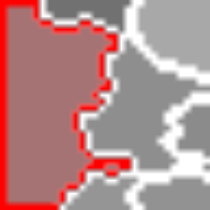
\includegraphics[width=.2\linewidth]{ipfs/ipfs-algorithms-nodesplitting-gui-a.png}}%
	%
	\hspace{8mm}%
	%
	\subfigure[Mark it to be split by clicking the menu item]
	{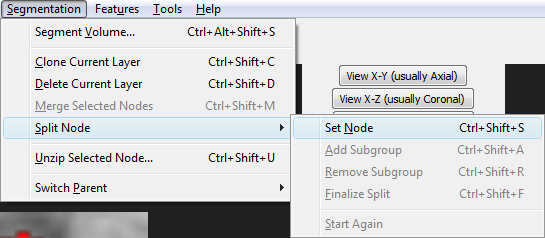
\includegraphics[width=.5\linewidth]{ipfs/ipfs-algorithms-nodesplitting-gui-b.png}}%
	%
	\hspace{8mm}%
	%
	\subfigure[After marking it, its children will be highlighted]
	{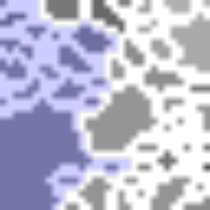
\includegraphics[width=.2\linewidth]{ipfs/ipfs-algorithms-nodesplitting-gui-c.png}}%
	%
	\hspace{8mm}%
	%
	\subfigure[Select the child nodes in a subgroup]
	{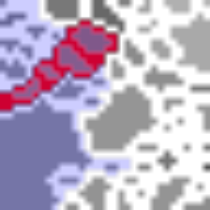
\includegraphics[width=.2\linewidth]{ipfs/ipfs-algorithms-nodesplitting-gui-d.png}}%
	%
	\hspace{8mm}%
	%
	\subfigure[Add the subgroup by clicking the menu item]
	{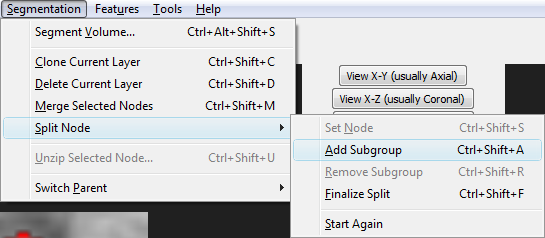
\includegraphics[width=.5\linewidth]{ipfs/ipfs-algorithms-nodesplitting-gui-e.png}}%
	%
	\hspace{8mm}%
	%
	\subfigure[Each subgroup will be assigned a different colour]
	{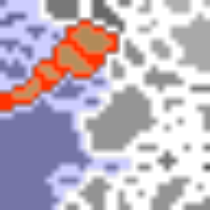
\includegraphics[width=.2\linewidth]{ipfs/ipfs-algorithms-nodesplitting-gui-f.png}}%
	%
	\hspace{8mm}%
	%
	\subfigure[Repeat (d)-(f) to add other subgroups, then finalize the split by clicking the menu item]
	{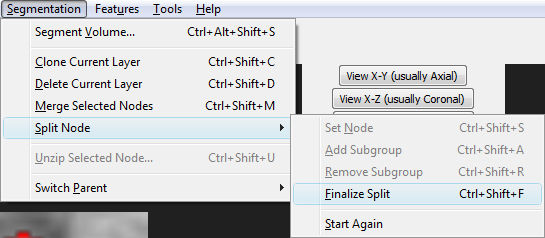
\includegraphics[width=.5\linewidth]{ipfs/ipfs-algorithms-nodesplitting-gui-g.png}}%
	%
	\hspace{8mm}%
	%
	\subfigure[The node will be split as indicated]
	{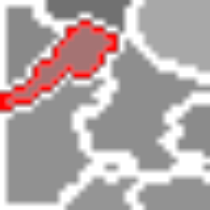
\includegraphics[width=.2\linewidth]{ipfs/ipfs-algorithms-nodesplitting-gui-h.png}}%
\caption{The user interface for node splitting}
\label{fig:ipfs-algorithms-nodesplitting-gui}
\end{stusubfig}
%---

\paragraph{Precondition Checking}

The following preconditions must be checked for node splitting (see the pseudo-code in Listing~\ref{code:ipfs-forest-splitnode} for the method):

\begin{enumerate}

\item The node to be split must not be in the leaf layer of the forest. (This can be trivially checked in $O(1)$ time.)
\item The node to be split must exist. (This can be checked in $O(1)$ time for the leaf layer, and $O(\log n_\ell)$ time for branch layer $\ell$.)
\item There must be more than one subgroup. (This can be trivially checked in $O(1)$ time.)
\item The subgroups must partition the children of the node being split. (This can be checked in time $O(\log C!)$, where $C$ is the number of children, since each inner loop iteration involves a logarithmic amount of work on a set whose size decreases linearly from $C$ to $1$, and $\sum_{i=1}^C \log i = \log C!$.)
\item Each of the subgroups must be non-empty and connected. (Each of the $G$ groups requires $O(1)$ time for the non-empty check, and TODO.)

\end{enumerate}

When implementing node splitting in a user interface like the one described above, these preconditions should be checked by the interface, not by the forest at the time of finalizing the split. The user should not, for example, have the option of adding invalid subgroups or finalizing a split without defining any subgroups.

\begin{stulisting}[p]
\caption{Forest : Split Node Precondition Checking}
\label{code:ipfs-forest-splitnode}
\begin{lstlisting}[style=Default]
function split_node
:	(node : NodeID; groups : Vector<Set<int>>;
	 checkPreconditions : CheckPreconditions) $\to$ Set<NodeID>

	if checkPreconditions = CHECK_PRECONDITIONS then
		// Check that the node to be split is not in the lowest layer.
		if node.layer() = 0 then throw;

		// Check that the node to be split is valid.
		var layer : BranchLayer? := checked_branch_layer(node.layer());
		if layer = null or not layer.has_node(node.index()) then throw;

		// Check that the groups partition the children of the node.
		var children : Set<int> := layer.node_children(node.index());
		for each group : Set<int> $\in$ groups
			for each childIndex : int $\in$ group
				if children.contains(childIndex) then
					children.erase(childIndex);
				else
					throw;
		if children $\ne$ {} then throw;

		// Check that each of the split groups is non-empty and connected.
		for each group : Set<int> $\in$ groups
			if group = {} then throw;
			if not are_connected(group, node.layer() - 1) then throw;

	// We only need to split the node if there's more than one group.
	if #groups $\ne$ 1 then
		var command : SplitNodeCommand := make_split_node_command(node, groups);
		command_manager().execute(command);
		return command.result();
	else
		var result : Set<NodeID>;
		result.insert(node);
		return result;
\end{lstlisting}
\end{stulisting}

\paragraph{Executing the Command}

Pseudo-code to execute a split node command is shown in Listing~\ref{code:ipfs-forest-splitnodeimpl}. TODO

\begin{stulisting}[p]
\caption{Forest : Split Node Implementation}
\label{code:ipfs-forest-splitnodeimpl}
\begin{lstlisting}[style=Default]
function split_node_impl
:	(node : NodeID; groups : Vector<Set<int>>) $\to$ Set<NodeID>

	var layerA : BranchLayer? := checked_branch_layer(node.layer() + 1);
	var layerS : BranchLayer := branch_layer(node.layer());
	var layerB : ForestLayer := forest_layer(node.layer() - 1);

	// Step 1: Delete the node being split from the forest.

	// Remove any forest links which reference the node.
	for each c : int $\in$ layerS.node_children(node.index())
		layerB.set_node_parent(c, -1);

	var parentIndex : int := layerS.node_parent(node.index());
	if layerA $\ne$ null then layerA.node_children(parentIndex).erase(node.index());

	// Remove the node from its partitioning graph.
	layerS.remove_node(node.index());

	// Step 2: Add new nodes for each of the groups to the split layer, along with
	// the appropriate forest links.
	var newNodes : Set<NodeID>;
	for each group : Set<int> $\in$ groups
		var groupIndex : int := lowest_int(group);	// note that group is non-empty
		newNodes.insert(NodeID(node.layer(), groupIndex));
		layerS.set_node_properties(groupIndex, layerB.combine_properties(group));
		layerS.set_node_children(groupIndex, group);
		layerS.set_node_parent(groupIndex, parentIndex);
		for each n : int $\in$ group
			layerB.set_node_parent(n, groupIndex);
		if layerA $\ne$ null then layerA.node_children(parentIndex).insert(groupIndex);

	// Step 3: Propagate the necessary edges from the child layer to the split layer.
	for each group : Set<int> $\in$ groups
		for each n : int $\in$ group
			for each e : Edge $\in$ layerB.adjacent_edges(n)
				var parentU : int := layerB.node_parent(e.u())
				var parentV : int := layerB.node_parent(e.v());
				if parentU $\ne$ parentV then
					layerS.update_edge_weight(parentU, parentV, e.weight());

	listeners.node_was_split(node, newNodes);
	return newNodes;
\end{lstlisting}
\end{stulisting}

\paragraph{Undoing the Command}

To undo a split node command, it is enough to just re-merge the results of the split using a sibling node merge (see Listing~\ref{code:ipfs-algorithms-mergesiblingnodesimpl} for pseudo-code).

\subsection{Zipping Algorithms}

Whilst the core mutating algorithms provide all that is theoretically required for partition forest editing, certain operations are nevertheless tedious for the user to perform using only these primitives. For instance, it seems intuitively sensible that the user should be able to merge not only nodes that are siblings in the forest, but any nodes that are adjacent in the graph for their forest layer. Such `higher-level' algorithms, however, require more substantial changes to the structure of the forest; in particular, they require changes to be made in more than one layer.

In order to facilitate the implementation of such algorithms, it is helpful to introduce two intermediary forest operations that I call \emph{unzip node} (or just \emph{unzipping}) and \emph{zip chains} (or just \emph{zipping}). These are respectively multi-layer split and merge operations on the forest, and can be implemented in terms of their lower-level counterparts. In fact, such an approach is not only possible but advisable, since it can be used to avoid writing special code to undo the operations. The key is to introduce an entity called a \emph{command sequence guard}. This is created at the start of a composite operation like an unzip, and informs the application's command manager that a command sequence is about to start (in C++, this would happen in the constructor for the guard). The relevant lower-level commands are then executed, after which the guard is destroyed again, informing the application's command manager that the command sequence has ended (in C++, this would happen in the guard's destructor). Undoing the composite operation is then a simple matter of undoing the lower-level commands in reverse order, something that can be easily handled by any decent command manager implementation. Bearing this in mind, we can now examine each of the zipping algorithms in detail.

\subsubsection{Unzipping}

\paragraph{Description}

A node in any layer of the hierarchy can be unzipped to a specified higher layer (or the top of the hierarchy). This essentially `separates out' the branch from the higher layer down to the specified node: it is effectively a multi-layer split, with a set containing the node in question as one of the groups at each stage. The key issue that has to be addressed in order to make this work is the need to find the other groups for each split: the algorithm presented here solves this problem by defining the other groups to be the connected components of what is left after removing the node being unzipped from consideration. See Figure~\ref{fig:ipfs-algorithms-unzipping} for an example.

% TODO: fig:ipfs-algorithms-unzipping

\paragraph{C++ Method Interface}

\begin{lstlisting}[style=Prototype]
typedef deque<NodeID> Chain;
vector<Chain> unzip_node(const NodeID& node, int toLayer);
\end{lstlisting}

\paragraph{User Interface for Image Analysis}

The user interface for unzipping is relatively straightforward, as illustrated in Figure~\ref{fig:ipfs-algorithms-unzipping-gui}. The user selects a node, then clicks a menu item to indicate that it should be unzipped. This brings up a dialog box that allows the user to choose the target layer of the unzip. After the user enters the target layer, the node is then unzipped as desired.

%---
\begin{stusubfig}{p}
	\subfigure[Layer 1 before unzipping]
	{
\includegraphics[width=.3\linewidth]{ipfs/ipfs-algorithms-unzipping-gui-a.png}}%
	%
	\hspace{8mm}%
	%
	\subfigure[Layer 2 before unzipping]
	{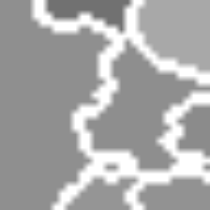
\includegraphics[width=.3\linewidth]{ipfs/ipfs-algorithms-unzipping-gui-b.png}}%
	%
	\\
	%
	\subfigure[Layer 3 before unzipping]
	{
\includegraphics[width=.3\linewidth]{ipfs/ipfs-algorithms-unzipping-gui-c.png}}%
	%
	\hspace{8mm}%
	%
	\subfigure[Select a node to unzip]
	{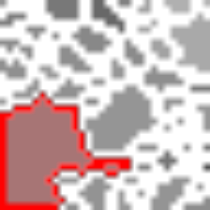
\includegraphics[width=.3\linewidth]{ipfs/ipfs-algorithms-unzipping-gui-d.png}}%
	%
	\\
	%
	\subfigure[Click the menu item]
	{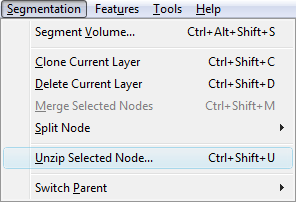
\includegraphics[width=.4\linewidth]{ipfs/ipfs-algorithms-unzipping-gui-e.png}}%
	%
	\hspace{8mm}%
	%
	\subfigure[Enter the target layer]
	{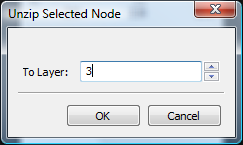
\includegraphics[width=.4\linewidth]{ipfs/ipfs-algorithms-unzipping-gui-f.png}}%
	%
	\\
	%
	\subfigure[Layer 2 after unzipping]
	{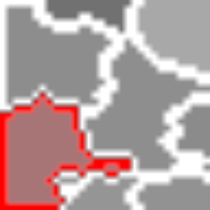
\includegraphics[width=.3\linewidth]{ipfs/ipfs-algorithms-unzipping-gui-g.png}}%
	%
	\hspace{8mm}%
	%
	\subfigure[Layer 3 after unzipping]
	{
\includegraphics[width=.3\linewidth]{ipfs/ipfs-algorithms-unzipping-gui-h.png}}%
\caption{The user interface for unzipping}
\label{fig:ipfs-algorithms-unzipping-gui}
\end{stusubfig}
%---

\paragraph{Precondition Checking}

The following preconditions must be checked for unzipping:

\begin{enumerate}

\item The node being unzipped must exist. (This can be checked in $O(1)$ time for the leaf layer, and $O(\log n_\ell)$ time for branch layer $\ell$.)
\item If $L$ is the layer containing the node being unzipped, and $H$ is the highest layer in the partition forest, then the index of the layer to which to unzip must be in the range $[L,H]$. (This can be trivially checked in $O(1)$ time.)

\end{enumerate}

\paragraph{Executing the Command}

TODO

\paragraph{Undoing the Command}

TODO

\subsubsection{Zipping}

\paragraph{Description}

TODO

\paragraph{C++ Method Interface}

\begin{lstlisting}[style=Prototype]
pair<NodeID,int> zip_chains(const vector<Chain>& chains);
\end{lstlisting}

\paragraph{User Interface for Image Analysis}

It doesn't make sense to expose zipping as part of the user interface, since the inputs it requires (node chains) are too cumbersome for the user to be asked to provide directly. More usable operations such as parent switching (described in the next section), that use zipping internally, should be exposed instead.

\paragraph{Precondition Checking}

TODO

\paragraph{Executing the Command}

TODO

\paragraph{Undoing the Command}

TODO

\subsection{Higher-Level Algorithms}

Having discussed unzipping and zipping in the previous section, we are now in a position to implement two higher-level partition forest algorithms that are of great practical use. The first of these is the previously-mentioned merging operation that allows the user to merge nodes based on their adjacency in their forest layer (i.e.~in an imaging context, their spatial adjacency within the image) rather than whether or not they share a common forest parent. As observed earlier, this is the `intuitive' merging operation that the user wants to perform on forest nodes (see e.g.~Figure~\ref{fig:ipfs-algorithms-nonsiblingnodemerging-motivation}), but it is a difficult operation to implement without the machinery provided by the zipping algorithms.

The second higher-level algorithm that we can now implement is parent switching, the problem tackled in a more constrained manner by Peter Nacken in \cite{nacken95}. TODO